\documentclass[12pt,pdftex]{article}
\usepackage[pdftex]{graphicx,color}
\usepackage{setspace,palatino,multirow}
\usepackage{amsmath,amssymb}
\usepackage{titlesec}
\usepackage{lscape}
%\usepackage{subfigure}
\usepackage{threeparttable}
\usepackage{natbib}
\bibliographystyle{ecta}
\usepackage{cite}
\usepackage{booktabs}
\usepackage{subcaption}
\usepackage{pdflscape}
\usepackage{afterpage}
\usepackage{xcolor}
\usepackage{rotating}
\usepackage[listings, most]{tcolorbox}
\definecolor{nblue}{RGB}{0,0,128}
\usepackage{afterpage}

\usepackage[pdftex,colorlinks=true, bookmarks=false,
pdfstartview={XYZ null null 0.85},
pdftitle={How Restrictive is U.S. Trade Policy?},
pdfauthor={Michael E. Waugh},
pdfkeywords={tariffs, trade wars, Minneapolis Fed, trade policy
Trade Restrictiveness Index, U.S. trade policy, Deadweight loss},
colorlinks=true,linkcolor=darkgray,citecolor=darkgray,urlcolor=darkgray,
breaklinks]{hyperref}


\newcounter{saveeqni}%
\newcounter{saveeqn01i}%
\newcommand{\alpheqni}{\setcounter{saveeqni}{\value{section}}%
%\setcounter{saveeqn01i}{\value{subsectioni}}%
\renewcommand{\theequation}
    {\alph{saveeqni}\mbox{.\arabic{equation}}}}%
\newcommand{\reseteqni}{\setcounter{equation}{\value{saveeqni}}%
\renewcommand{\theequation}{\arabic{equation}}}%

\newtheorem{as}{Assumption}
\newtheorem{reg}{Regularity Condition}
\newtheorem{conjecture}{Conjecture}
\newtheorem{corr}{Corollary}
\newtheorem{df}{Definition}
\newtheorem{lemma}{Lemma}
\newtheorem{prp}{Proposition}
\newtheorem{rmk}{Remark}
\newenvironment{prf}{{\bf Proof}}{\hfill { }}

\DeclareMathOperator*{\plim}{plim}
\DeclareMathOperator*{\umax}{max}

\special{papersize=8.5in,11in}
\onehalfspacing
\setlength{\parindent}{0.1em}
\setlength{\parskip}{.09in}
\textwidth15.75cm
\evensidemargin 1.5in
\oddsidemargin 1.5in
\topmargin 8.5cm
\textheight 10in
\hyphenation{over-lapping}

\tcolorboxenvironment{prp}{%
boxrule = 0mm, breakable, colframe=white,
before skip=5pt,after skip=5pt,
colback=gray!5!white,
top = 2mm,
bottom = 2mm%,
%borderline north={1pt}{1pt}{gray},
%borderline south={1pt}{1pt}{gray}
}

\titleformat{\section}{\color{black}\large\bf}{\color{black}{\thesection.}}{.25cm}{}
\titleformat{\subsection}{\color{black}\normalsize\bf}{\thesubsection.}{.5em}{}
\titleformat{\subsubsection}{\color{black}\normalsize\bf}{\thesubsubsection.}{.5em}{}

\titlespacing{\section}{0pt}{*1.5}{*.5}
\titlespacing{\subsection}{0pt}{*1.5}{*.5}
\titlespacing{\subsubsection}{0pt}{*1.5}{*.5}

\def\thesection{\arabic{section}}
\def\thesubsection{\arabic{section}.\arabic{subsection}}
\def\thesubsubsection{\arabic{section}.\arabic{subsection}.\Alph{subsubsection}}

\def\citeapos#1{\citeauthor{#1}'s (\citeyear{#1})}

\renewcommand{\arraystretch}{1.1}
\usepackage[margin=2cm]{geometry}

\newcommand{\rmsValuetwofive}{15}
\newcommand{\meanWeightedValuetwofive}{8}
\newcommand{\simpleMeanValuetwofive}{6}
\newcommand{\currentdate}{July 2026}
\newcommand{\diffmeanWeightedValuetwofive}{7}
\newcommand{\diffsimpleMeanValuetwofive}{9}
\newcommand{\rmsValuetwofour}{7}
\newcommand{\meanWeightedValuetwofour}{3}
\newcommand{\simpleMeanValuetwofour}{3}
\newcommand{\olddate}{July 2024}
\newcommand{\peakdate}{October 2025}
\newcommand{\rmsValuepeak}{23}
\newcommand{\meanWeightedValuepeak}{14}
\newcommand{\simpleMeanValuepeak}{11}
\newcommand{\prerulingdate}{February 2026}
\newcommand{\rmsValuepreruling}{18}
\newcommand{\meanWeightedValuepreruling}{11}
\newcommand{\simpleMeanValuepreruling}{9}
\newcommand{\canadarmsValuetwofive}{11}
\newcommand{\canadameanWeightedValuetwofive}{4}
\newcommand{\canadasimpleMeanValuetwofive}{3}
\newcommand{\mexicormsValuetwofive}{9}
\newcommand{\mexicomeanWeightedValuetwofive}{4}
\newcommand{\mexicosimpleMeanValuetwofive}{3}
\newcommand{\chinarmsValuetwofive}{26}
\newcommand{\chinameanWeightedValuetwofive}{19}
\newcommand{\chinasimpleMeanValuetwofive}{21}


\newcommand{\rmsValuetwofiveMachinery}{12}
\newcommand{\meanWeightedValuetwofiveMachinery}{7}
\newcommand{\simpleMeanValuetwofiveMachinery}{3}
\newcommand{\rmsValuetwofiveElectricalEquipment}{12}
\newcommand{\meanWeightedValuetwofiveElectricalEquipment}{6}
\newcommand{\simpleMeanValuetwofiveElectricalEquipment}{5}
\newcommand{\rmsValuetwofiveVehicles}{15}
\newcommand{\meanWeightedValuetwofiveVehicles}{12}
\newcommand{\simpleMeanValuetwofiveVehicles}{13}
\newcommand{\rmsValuetwofivePharmaceuticals}{1}
\newcommand{\meanWeightedValuetwofivePharmaceuticals}{0}
\newcommand{\simpleMeanValuetwofivePharmaceuticals}{0}


\begin{document}


\begin{onehalfspacing}

{\large \textbf{How Restrictive is U.S. Trade Policy?}}

\vspace{0.5cm}

\href{http://www.waugheconomics.com/}{Michael E. Waugh} \\ Federal Reserve Bank of Minneapolis and NBER

\vspace{0.5cm}

February 2026

\vspace{0.5cm}

Most Recent Data: \textbf{\currentdate{}}

\vspace{1.5cm}


\normalsize

ABSTRACT ------------------------------------------------------------------------------------------------------------

This short note computes Trade Restrictiveness Index measures for current U.S. trade policy. Building on the ideas of \citet{anderson1996new, anderson2005measuring}, the Trade Restrictiveness Index is the uniform tariff that leaves the U.S. consumer as well off as under actual policy. As of \currentdate{}, U.S. trade policy is twice as restrictive as headline tariff numbers suggest. The Trade Restrictiveness Index is \rmsValuetwofive{}  percent, which stands in contrast to the \simpleMeanValuetwofive{} percent average tariff rate. Trade policy towards Canada and Mexico is two to three times more restrictive than average tariff rates suggest. Sectoral analysis shows that the restrictiveness is concentrated in vehicles, machinery, and electrical equipment.

------------------------------------------------------------------------------------------------------------------------------
\vspace{0.25cm}

JEL Classification: F13, F14\\
%%
%%
Keywords: Tariffs, U.S. Trade Policy, Trade Restrictiveness Index

% need to run notebooks: TRI-all-country.ipynb
% then run TRI-sector

\vspace{4.0cm}

{\footnotesize Email: michael.e.waugh@gmail.com. The views expressed herein are those of the author and not necessarily those of the Federal Reserve Bank of Minneapolis or the Federal Reserve System. My github repository provides the code and supplementary work behind this paper at \url{https://github.com/tradewartracker/how-restrictive-us-trade}.}

\hspace{-0.05cm}

\newpage

\subsection*{Introduction}

Since January 2025, trade policy in the U.S. has changed dramatically with large and heterogeneous increases in tariff rates. This short note asks the following question: How restrictive is current U.S. trade policy? My answer is that it is roughly twice as restrictive as the headline average tariff statistics suggest.

Two features of current policy make averages misleading. First, the heterogeneity in tariff rates---both across countries and products---means that averages will understate the overall restrictiveness of U.S. trade policy. The reason is that the deadweight loss from a tariff increases with the \emph{square} of the tariff rate, not linearly. This implies that, in aggregate, two tariff regimes with the same average tariff but differences in the variance of tariffs have different economic consequences. Put simply: a few very high tariffs create more distortions than many moderate tariffs with the same average rate.

To address this challenge, I utilize the ideas of \citet{anderson1996new, anderson2005measuring}, who index how restrictive trade policy is by the uniform tariff that, when applied to all goods, leaves the U.S. consumer as well off as under the actual, heterogeneous tariffs. In general, implementing this approach is not a trivial task and requires a full general-equilibrium model. Instead, I employ the quadratic approximation developed by \citet{feenstra1995estimating} and \citet*{keeNicitaOlarreaga2009}, resulting in an easily implementable measure of trade restrictiveness which is the trade-weighted, root-mean-square of tariffs. \citet{irwin2010trade} applies this framework to historical U.S. tariffs; I extend the approach to current U.S. trade policy.

The second challenge is the following---what \emph{is} U.S. trade policy? The issue is that a simple, numerical statement about the tariff is sometimes not possible. For example, whether a U.S. importer from Mexico faces a tariff depends upon whether that importer has shown that the product is covered under the United States-Mexico-Canada Trade Agreement (USMCA). As another example, many products imported from Brazil are tariffed or not depending upon whether they ultimately go into civilian aircraft. The steel and aluminum tariffs extend to derivative products, but only their steel and aluminum content is tariffable. And the list goes on.

To address this concern, I infer applied tariffs from data on duties collected, rather than constructing statutory tariffs. Specifically, I use the public Census trade data, which reports duty collected and values at the 10-digit Harmonized System level, by country. This approach allows me to infer the \emph{de facto} applied tariff rate for each product-country pair. This is in contrast to trying to measure the \emph{de jure} tariffs by following the announced statutes and then making assumptions about how they might be implemented.\footnote{\citet{tracker} (\url{https://www.tradewartracker.com}) or \citet{budgetlab2025tariffs} are examples that try and construct estimates of the weighted average tariff given the announced statutes.}

Using the de facto tariffs, I compute trade restrictiveness indices in aggregate, by U.S. trading partner, and by sector. Two main results emerge from this analysis. First, in aggregate, current U.S. trade policy (as of \currentdate{}) has a Trade Restrictiveness Index (TRI) of \rmsValuetwofive{} percent. That is, a \rmsValuetwofive{} percent uniform tariff yields the same deadweight loss as current trade policy. In contrast, the average tariff rate (tariff revenue divided by imports) is \simpleMeanValuetwofive{} percent. Current U.S. trade policy is more restrictive than it appears.

The second important result is that for certain countries, U.S. trade policy is significantly more restrictive than what it appears to be. Canada and Mexico are the most important examples, with trade restrictiveness indices of \canadarmsValuetwofive{} and \mexicormsValuetwofive{} percent, respectively. In contrast, average tariff rates are \canadasimpleMeanValuetwofive{} and \mexicosimpleMeanValuetwofive{} percent.

The issue here is that most trade with these countries face zero tariffs under the USMCA, but the tariffs that are applied | concentrated on products like autos and metals | are important and create substantial distortions that averages fail to capture. I confirm this point by computing Sectoral TRIs and find that vehicles face a high level of trade restrictiveness equivalent to a uniform tariff of roughly \rmsValuetwofiveVehicles{} percent.

These distinctions matter for policy and future trade negotiations. Trade restrictiveness indices are used by international institutions to monitor trade policy and by negotiators to evaluate whether proposed concessions represent genuine liberalization or not. A country can lower average tariffs while maintaining a high TRI by offering reductions on low-volume products while keeping high tariffs on key sectors.  Current U.S. trade policy towards Canada and Mexico is a case in point. And the sectoral TRIs make clear that high tariffs are concentrated in specific sectors.

\section{Trade Restrictiveness in Theory}\label{sec:theory}

This section describes the theoretical framework behind the measurement of the trade restrictiveness indices presented in Section \ref{sec:data}. The framework below builds on ideas in \citet{anderson1996new, anderson2005measuring}, who define a Trade Restrictiveness Index (TRI) as the uniform tariff that, when applied to all goods, leaves the representative household as well off as under the actual vector of trade distortions.

As discussed in \citet{keeNicitaOlarreaga2009}, the Anderson--Neary measure faces several difficulties in practice. In line with their approach, I construct a second-order, welfare-consistent approximation to the TRI, relying on a Harberger-style quadratic expansion of the welfare loss. This derivation is closely related to the treatment in \citet{feenstra1995estimating}. This approximation avoids the computational burden of the full Anderson--Neary CGE approach, which requires specifying production functions, preference parameters, factor markets, and numerically solving for general equilibrium prices. Instead, the approximation requires only observable data on tariffs, import shares, and (possibly) elasticities of import demand.

\subsection{The Deadweight Loss of Tariffs}

The environment considered is one in which there are many goods indexed $g=1,\dots,G$. The government levies ad valorem tariffs $\tau_{g,t}$ on each good, at date $t$. The framework applies to any definition of a ``good.'' In the empirical implementation, I define goods at the HS10-by-country level, treating the same product from different countries as distinct goods facing potentially different tariffs.

The goal is to summarize the entire vector $\{\tau_{g,t}\}_{g=1}^G$ with a \textbf{\emph{single}} uniform tariff rate $\hat{\tau}_{t}$, such that the uniform tariff has the same welfare impact as the structure of actual tariffs. To operationalize this idea, I employ a Harberger-style deadweight-loss formula, first for an individual good and then aggregated across all goods.

The Harberger triangle formula associated with a tariff on good $g$ is
\begin{align}
  \Delta W_{g,t} \approx \frac{1}{2}\,\theta_{g,o}\,\tau_{g,t}^2\,M_{g,o},
  \label{eq:dw_single}
\end{align}
where $M_{g,o}$ is import expenditure and $\theta_{g,o}$ is the (absolute value of the) compensated import demand elasticity, all evaluated at the initial equilibrium with the subscript $o$ indexing initial values. The subscript $t$ indexes the policy at date $t$. In the Appendix, I show that an alternative derivation based on a second-order expansion of the expenditure function yields the same results.

I then aggregate (\ref{eq:dw_single}) across all goods and arrive at the \textbf{aggregate} deadweight loss from the tariff vector $\{\tau_{g,t}\}$
\begin{align}
  \Delta W_t \approx \frac{1}{2} \sum_{g=1}^G \theta_{g,o} \tau_{g,t}^2 M_{g,o}.
  \label{eq:dw_agg}
\end{align}
This deadweight loss calculation can then be expressed as a weighted average of the square of tariffs:
\begin{align}
\Delta W_t \approx & \frac{1}{2} A_o \sum_{g=1}^G \omega_{g,o} \tau_{g,t}^2, \label{eq:dw_agg_weights} \\
\nonumber \\
\quad \mbox{where} \quad A_{o} \equiv \sum_{g'=1}^G \theta_{g',o} M_{g',o} &\quad \mbox{and} \quad \omega_g \equiv \frac{\theta_{g,o} M_{g,o}}{\sum\limits_{g'=1}^G \theta_{g',o} M_{g',o}}. \nonumber
\end{align}
The weights in (\ref{eq:dw_agg_weights}) reflect two issues: (i) how sensitive good $g$ is to a change in price | this is the elasticity $\theta_{g,o}$ part; and (ii) how important good $g$ is as measured by import expenditure $M_{g,o}$.

\subsection{The Uniform Tariff Equivalent}

Following the Anderson--Neary logic, I want to find the uniform tariff | $\hat{\tau}_{t}$ | which leads to the same aggregate deadweight loss as in (\ref{eq:dw_agg_weights}). Under a uniform tariff, the deadweight loss is
\begin{align}
\Delta W^{uni}_t \approx \frac{1}{2} A_{o}\, \hat{\tau}_{t}^2.
\label{eq:uniform_dw}
\end{align}
where the $A_{o}$ term is defined the same as in (\ref{eq:dw_agg_weights}). Then equating (\ref{eq:uniform_dw}) and (\ref{eq:dw_agg_weights}) gives
\begin{align}
\hat{\tau}_{t} = \sqrt{\sum_{g=1}^G \omega_{g,o} \tau_{g,t}^2},
\label{eq:TRI1}
\end{align}
where the uniform tariff equivalent is the weighted, root-mean-square tariff.

I'll make one more assumption to simplify things | I'll abstract from heterogeneity in elasticities, so $\theta_{g,o} = \bar \theta$. This is a strong assumption and deviates from \citeapos{keeNicitaOlarreaga2009} approach, which estimates good-specific elasticities. The appeal here is that measurement is simplified dramatically. Under the common import demand elasticity assumption, the uniform tariff simplifies to
\begin{equation}
\hat{\tau}_t = \sqrt{\sum_{g=1}^G s_{g,o} \tau_{g,t}^2}, \quad \quad \mbox{where} \quad s_{g,o} \equiv \frac{M_{g,o}}{\sum\limits_{g'=1}^G  M_{g',o}}.
\label{eq:TRI2}
\end{equation}
Under this assumption, the uniform tariff is an import-share-weighted, root-mean-square of actual tariffs. This provides a back-of-the-envelope index that captures in one number how restrictive or not a tariff regime is and in a theoretically consistent way. For the rest of the paper, I'll refer to $\hat \tau$ in (\ref{eq:TRI2}) as the Trade Restrictiveness Index (TRI).

\subsection{Alternative Aggregate Tariff Measures}

I'll contrast the TRI with two alternative tariff measures. The first one is the mean weighted tariff which is
\begin{equation}
\bar{\tau}_{t} = \sum_{g=1}^G s_{g,o} \tau_{g,t}
\label{eq:average_tariff}
\end{equation}
where the weights $s_g$ are the same as in the TRI measure in (\ref{eq:TRI2}). Throughout the rest of the paper, I'll refer to $\bar{\tau}$ in (\ref{eq:average_tariff}) as the mean weighted tariff.

Under the assumption of common import demand elasticities, the mean weighted average tariff can also be interpreted as \citeapos{anderson2003mercantilist} Mercantilist Index of Trade Policy (MTRI). The MTRI answers the question: what uniform tariff would leave aggregate imports at their current level? As shown in \citet{keeNicitaOlarreaga2009}, the MTRI is just a weighted average tariffs where the weights are the same as discussed in (\ref{eq:dw_agg_weights}). And with common import demand elasticities, the weights are simply the import shares.

The TRI connects with the mean weighted tariff through the following relationship
\begin{align}
\hat{\tau}_{t} = \bar{\tau}_{t}\sqrt{1 + \sigma_{\tau,t}^2}, \quad \mbox{where} \quad \sigma_{\tau,t}^2 = \sum\limits_{g=1}^G s_{g,o}\bigg(\frac{\tau_{g,t} - \bar{\tau_{t}}}{\bar{\tau_{t}}}\bigg)^2
\label{eq:TRI3}
\end{align}
where the $\sigma_{\tau,t}$ term is the import-weighted variance of tariffs, measured as percent deviations from the mean. This means that for a given average tariff, a regime with high tariff dispersion | such as one with many exemptions and a few very high rates | will be substantially more restrictive than the average suggests. As I discuss in Section \ref{sec:results1}, this is precisely the situation with current U.S. policy toward Canada and Mexico.

Another commonly used metric is the total value of duties collected divided by the total value of imports or
\begin{equation}
\tilde{\tau}_{t} = \frac{\sum\limits_{g=1}^G M_{g,t}\tau_g}{\sum\limits_{g'=1}^G  M_{g',t}} \quad = \quad \sum_{g=1}^G s_{g,t} \tau_{g,t}. \label{eq:duty_tariff}
\end{equation}
I'll refer to $\tilde{\tau}$ as in (\ref{eq:duty_tariff}) as the duty / imports tariff rate. The last line makes clear that this is a weighted average tariff | just that the weights are varying with the date (the $s$'s are indexed by $t$, not the original pre-tariff point at $o$). While widely used, it is problematic because the weights will typically fall on the goods with the largest tariffs as firms and consumers substitute away. Thus, this measure will tend to understate how restrictive trade policy is relative to the mean weighted or TRI tariff measures.


%inally, this measure can be decomposed into a mean and variance component. Define the mean and variance component as
%\begin{align}
%&\underbrace{\bar{\tau} = \sum_{g=1}^G s_g \tau_g}_{\small\mbox{Mean Tariff}} \quad \mbox{and} \quad \underbrace{\sigma_{\tau}^2 = \sum_{g=1}^G s_g\bigg(\frac{\tau_g - \bar{\tau}}{\bar{\tau}}\bigg)^2}_{\small\mbox{Variance of Tariffs}}.
%\label{eq:mean_variance}
%\end{align}
%Where the first term is a simple, weighted average tariff. The second component is the variance of the tariffs which is expressed in percent deviations from the average tariff. Given these measures, I can reexpress (\ref{eq:TRI2}) in terms of the mean and variance:
%\begin{align}
%\hat{\tau} = \bar{\tau}\sqrt{1 + \left(\sigma_{\tau}\right)^2}.
%\label{eq:TRI3}
%\end{align}
%Expressed in this form, (\ref{eq:TRI3}) highlights how dispersion in tariff rates is costly. Condition on the mean tariff rate, the uniform tariff required to match the same deadweight loss is increasing in the variance of the tariffs. Put more simply, more dispersed tariffs are more restrictive than less dispersed tariffs.

\section{Measuring Trade Restrictiveness}\label{sec:data}

This section details how I measure the objects in (\ref{eq:TRI2}) in the data. My main data source is the U.S. Census FT900 U.S. International Trade in Goods and Services data release and specifically the Monthly International Trade Datasets. These data provide detail on U.S. imports and the duty collected at the Harmonized System (HS) 10 digit level, by country, at the monthly frequency. The Census API only has the Monthly Datasets dating back to 2013 and thus is the start of the time series that I consider.

\subsection{Measuring Tariffs and Weights}

As mentioned in the introduction, my main approach is to infer tariffs from the data rather than follow the statutes and make assumptions about how they are implemented or the extent to which some firms are subject to tariffs or not. Specifically, I measure tariffs by computing
\begin{align}
\tau_{g,t} = \frac{\mbox{duties collected on imports $g$ for consumption}_{t}}{\mbox{value of imports of $g$ for consumption}_{t}}, \label{eq:realized-tariff}
\end{align}
or the ratio of the dutiable value of imports for consumption relative to the value of imports for consumption. The inferred tariff represents the average effective tariff rate actually paid by importers of good $g$. This corresponds to $\tau_{g,t}$ in the theoretical framework, where the relevant tariff for welfare calculations is the rate importers actually face, not the statutory rate that may or may not apply depending on exemptions.

The definition of a good $g$ will depend upon the context, so when I analyze overall or sectoral trade restrictiveness it will be a country-by-HS10-code. When I analyze country-specific TRIs, the country dimension is no longer relevant and it is just an HS10-code.

What this approach will do is infer the extent to which some importers are able to claim exemptions, as well as the tariffable content embedded in the ``typical product.'' For example, importers that are non-USMCA compliant would face a tariff of 25 percent when importing from Mexico. In this example, when I infer the tariff, it will reflect an average of (i) importers who are compliant and thus face the USMCA tariff and (ii) importers who are not-compliant and face the 25 percent tariff. The data reveals the division between (i) and (ii), not myself or other researchers making this ex-ante choice.

The weights $s_{g,o}$ are measured in a similar way. They are the annual value of imports for a good divided by the total annual value of all imports in the year 2024. As mentioned above, a good is either the cross of a country by HS10 code or just an HS10 code in the country-specific contexts.


\section{The Restrictiveness of U.S. Trade Policy}\label{sec:results1}

Figure \ref{fig:tariff-histogram} shows how restrictive U.S. trade policy has become. In both panels, I report a histogram of tariffs for two time periods: \olddate{} and \currentdate{}. The unit of observation here is the tariff associated with an HS10 code and country. The y-axis reports the share of U.S. imports that lies within each particular bin. Three vertical lines are shown which demarcate the three aggregate tariff measures discussed above: (i) the TRI tariff defined in (\ref{eq:TRI2}), (ii) the mean weighted tariff in (\ref{eq:average_tariff}), and (iii) duty divided by imports in (\ref{eq:duty_tariff}).

\begin{figure}[p]
\centering
\caption{The Distribution of Tariffs (HS10 by Country)\\}\label{fig:tariff-histogram}
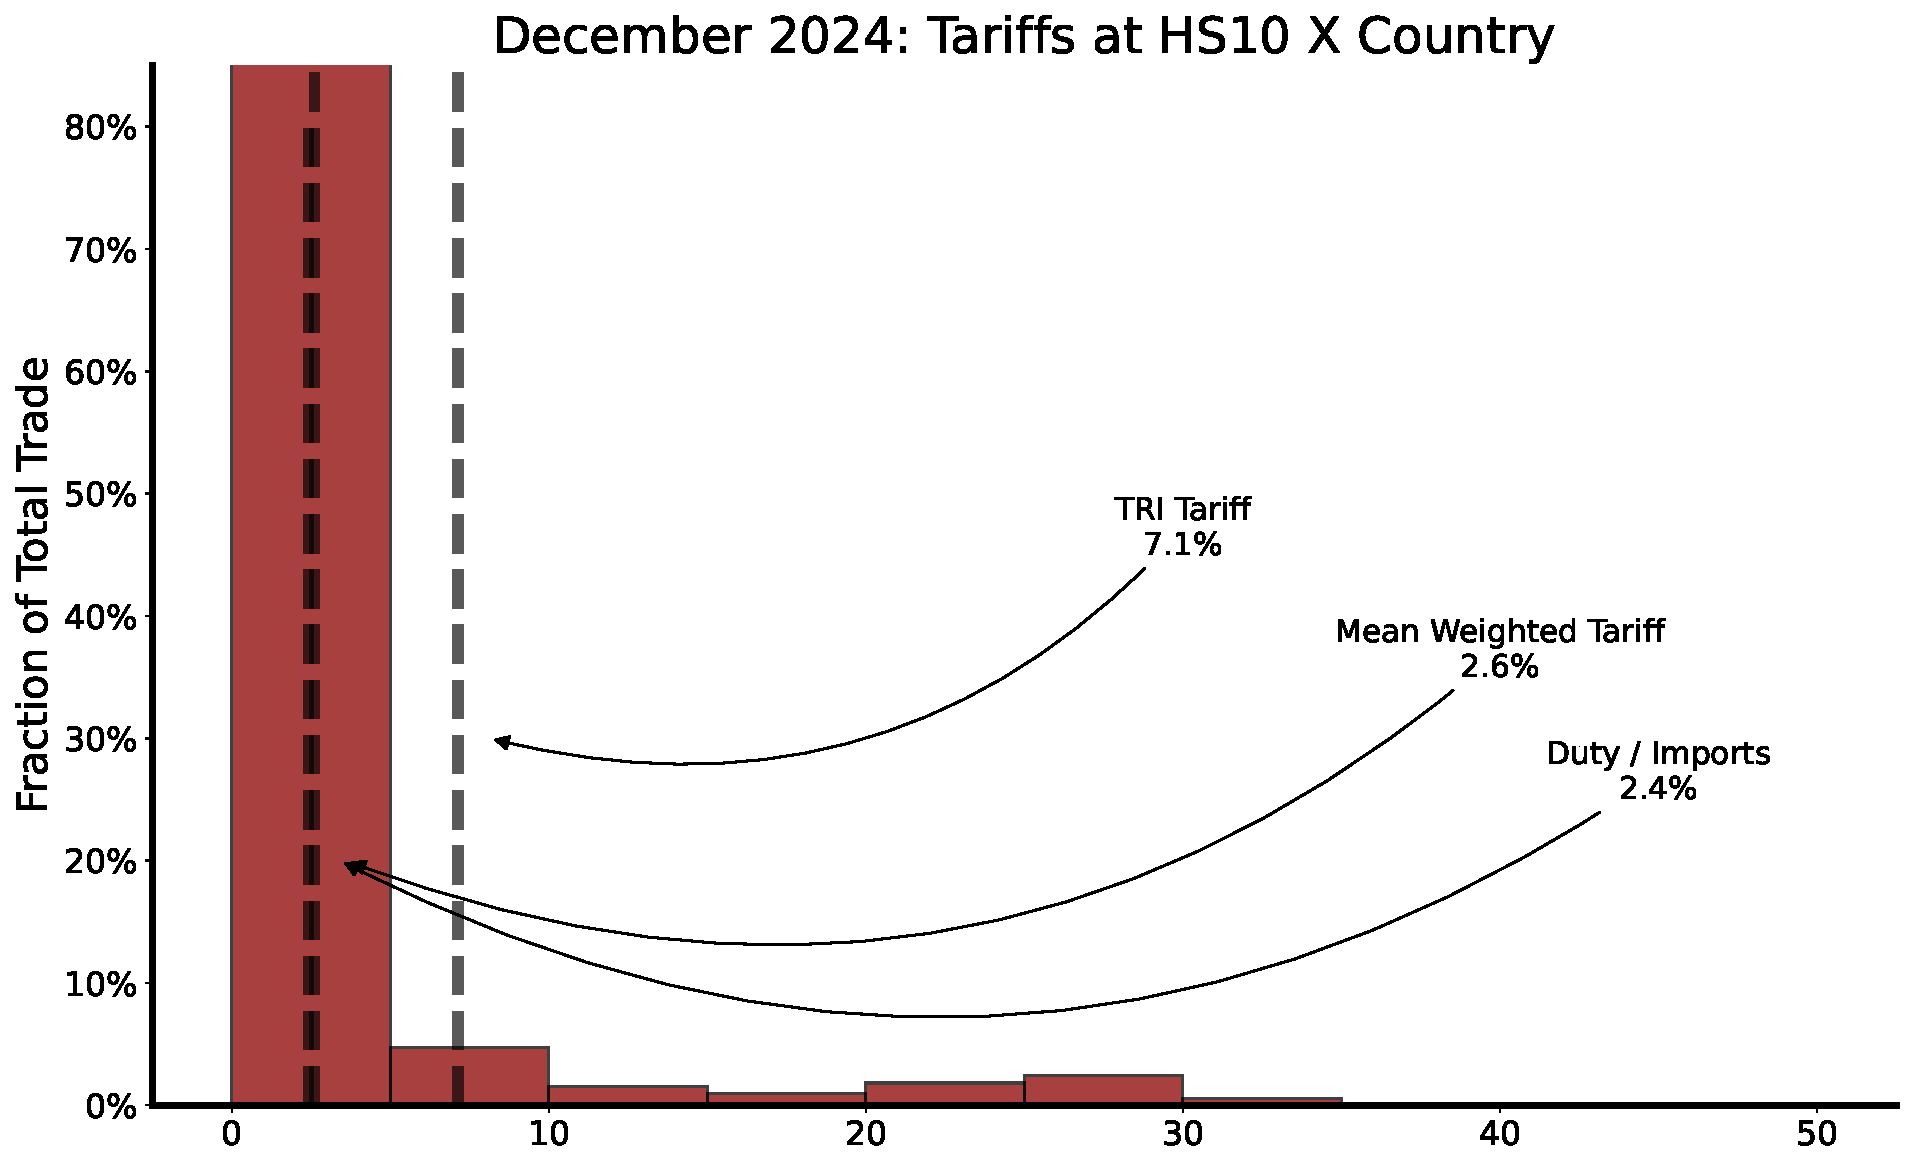
\includegraphics[height=0.45\textheight]{./figures/2024-12-histogram.pdf}\label{foo}\\[0.5em]
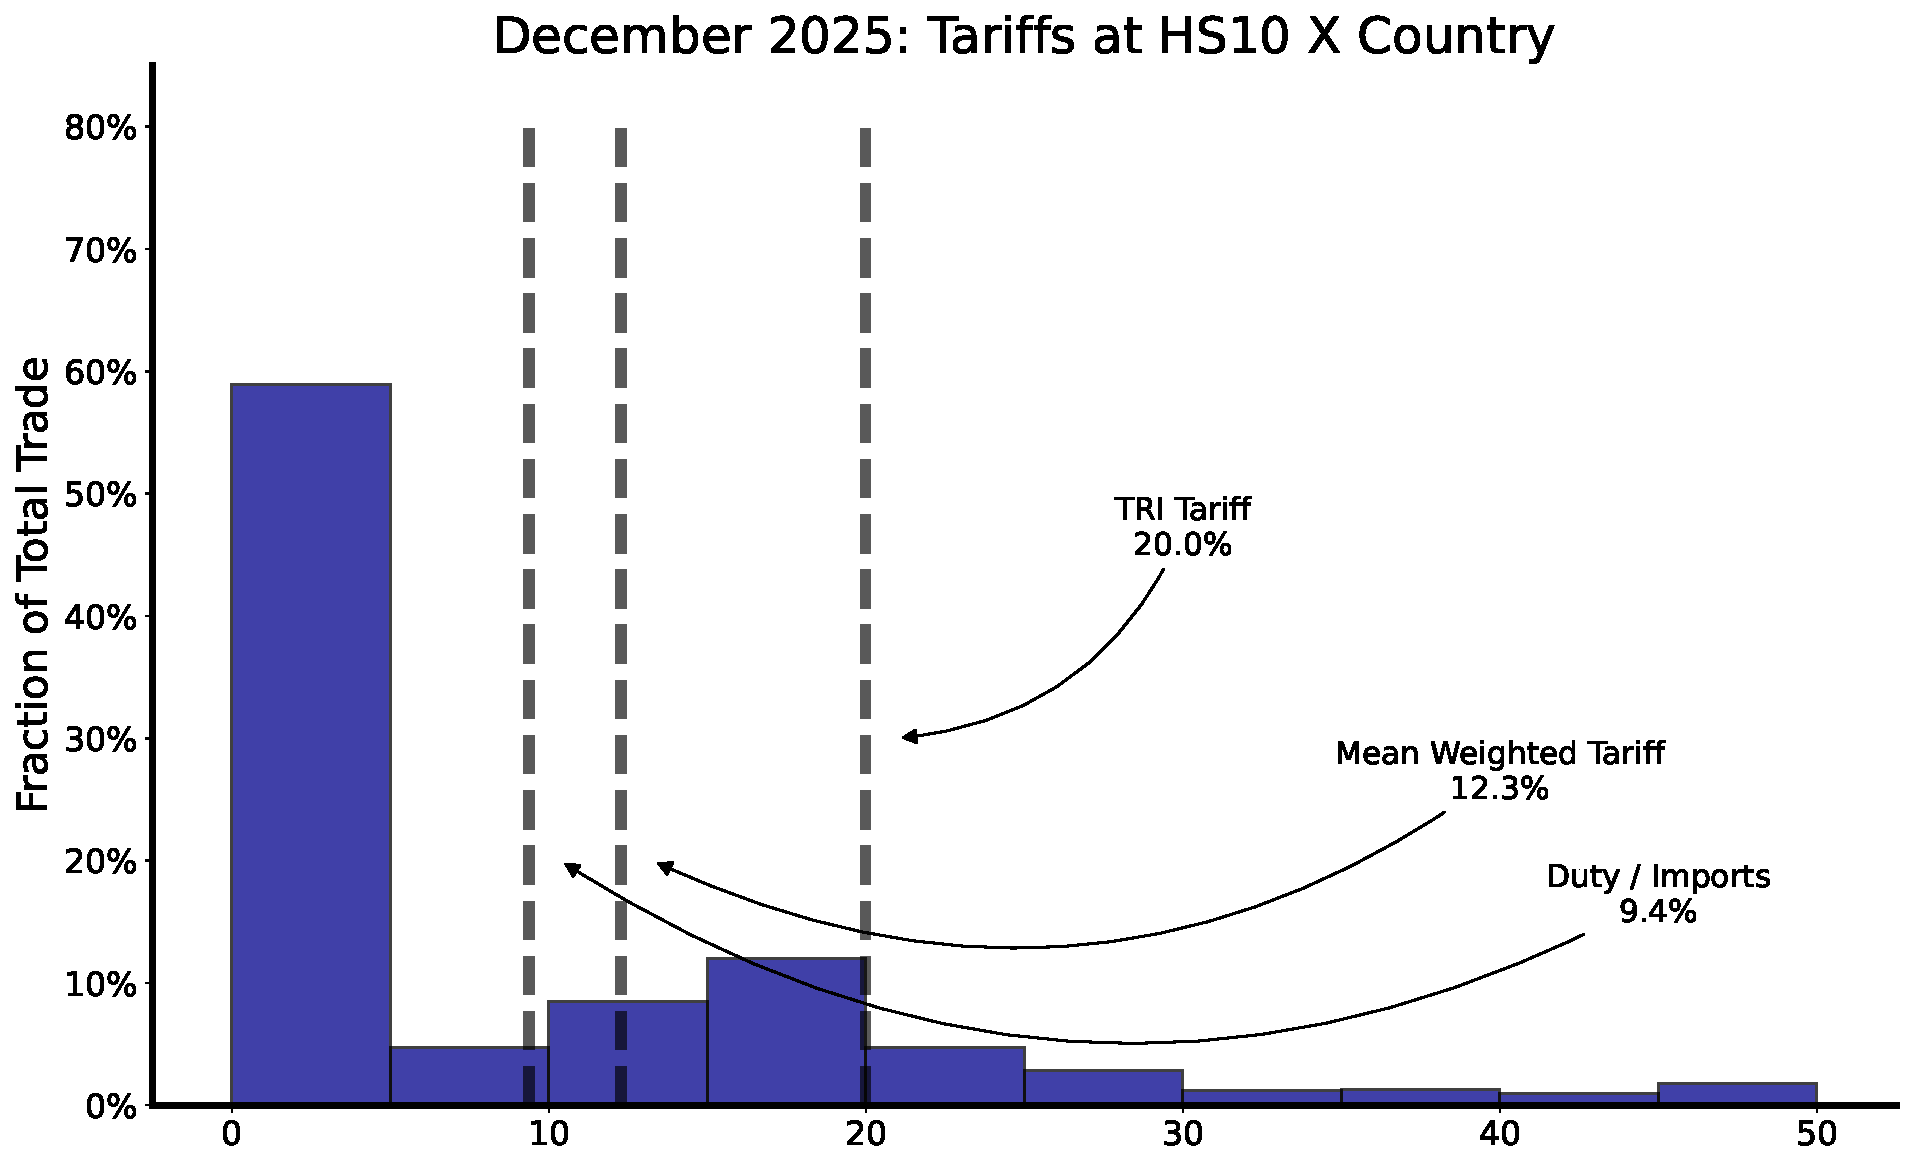
\includegraphics[height=0.45\textheight]{./figures/2025-12-histogram.pdf}
\end{figure}

In \olddate{}, mean tariffs were low at \simpleMeanValuetwofour{} percent and nearly 75 percent of trade was being imported with near zero tariffs. However, there is meaningful dispersion in tariffs for the remaining 25 percent of imports. And this dispersion leads to a TRI tariff measure of \rmsValuetwofour{} percent.

The bottom panel of Figure \ref{fig:tariff-histogram} reports the most recent month available, \currentdate{}. It starkly illustrates how much more restrictive U.S. trade policy has become.

The most important observation is that U.S. trade policy is substantially more restrictive than average rates would suggest. The TRI tariff currently stands at \rmsValuetwofive{} percent, more than \diffsimpleMeanValuetwofive{} percentage points larger than what the duty / imports tariff rate of \simpleMeanValuetwofive{} percent would imply, and \diffmeanWeightedValuetwofive{} percentage points larger than the mean weighted tariff of \meanWeightedValuetwofive{}.\footnote{As a separate observation, the mean weighted tariff does not differ markedly from measures using the announced statutory rates. For example, \citet{tracker} (\url{https://www.tradewartracker.com}) or \citeauthor{budgetlab2025tariffs} report weighted tariff rates of between 15 and 17 percent depending upon the exact month looked at versus \meanWeightedValuetwofive{} using tariffs inferred from the Census data.} Recall that the TRI is the uniform tariff that would generate the same aggregate welfare loss as the actual tariff structure. A TRI of \rmsValuetwofive{} percent means that current policy | with its mix of exemptions and high rates | is as costly to U.S. consumers as a uniform \rmsValuetwofive{} percent tariff on all imports.

The key issue is that current U.S. trade policy is generating a large amount of dispersion in tariff rates, even though the average tariff rate might seem modest. The histogram illustrates the point by highlighting how large amounts of U.S. imports are subject to tariff rates exceeding 10 or even 20 percent. The TRI tariff recognizes that the welfare cost of these higher tariff rates increases quadratically. Thus, the uniform tariff required to deliver the same deadweight loss as the current tariff regime is significantly larger than what other tariff measures would imply.

\subsection{Over time and Across Countries}\label{sec:results2}

The histograms in Figure \ref{fig:tariff-histogram} hide interesting variation both across time and countries. Figure \ref{fig:tariff-pannel} illustrates this point by plotting different tariff measures for the top 3 U.S. trading partners since the beginning of 2025 and the All Country aggregate. Table \ref{tab:tariff_metrics} reports tariff metrics for the top 20 U.S. trading partners as of \currentdate{}.

\afterpage{%
\clearpage
\begin{landscape}
\begin{figure}
\centering
\caption{Tariff Measures for Selected Countries}\label{fig:tariff-pannel}
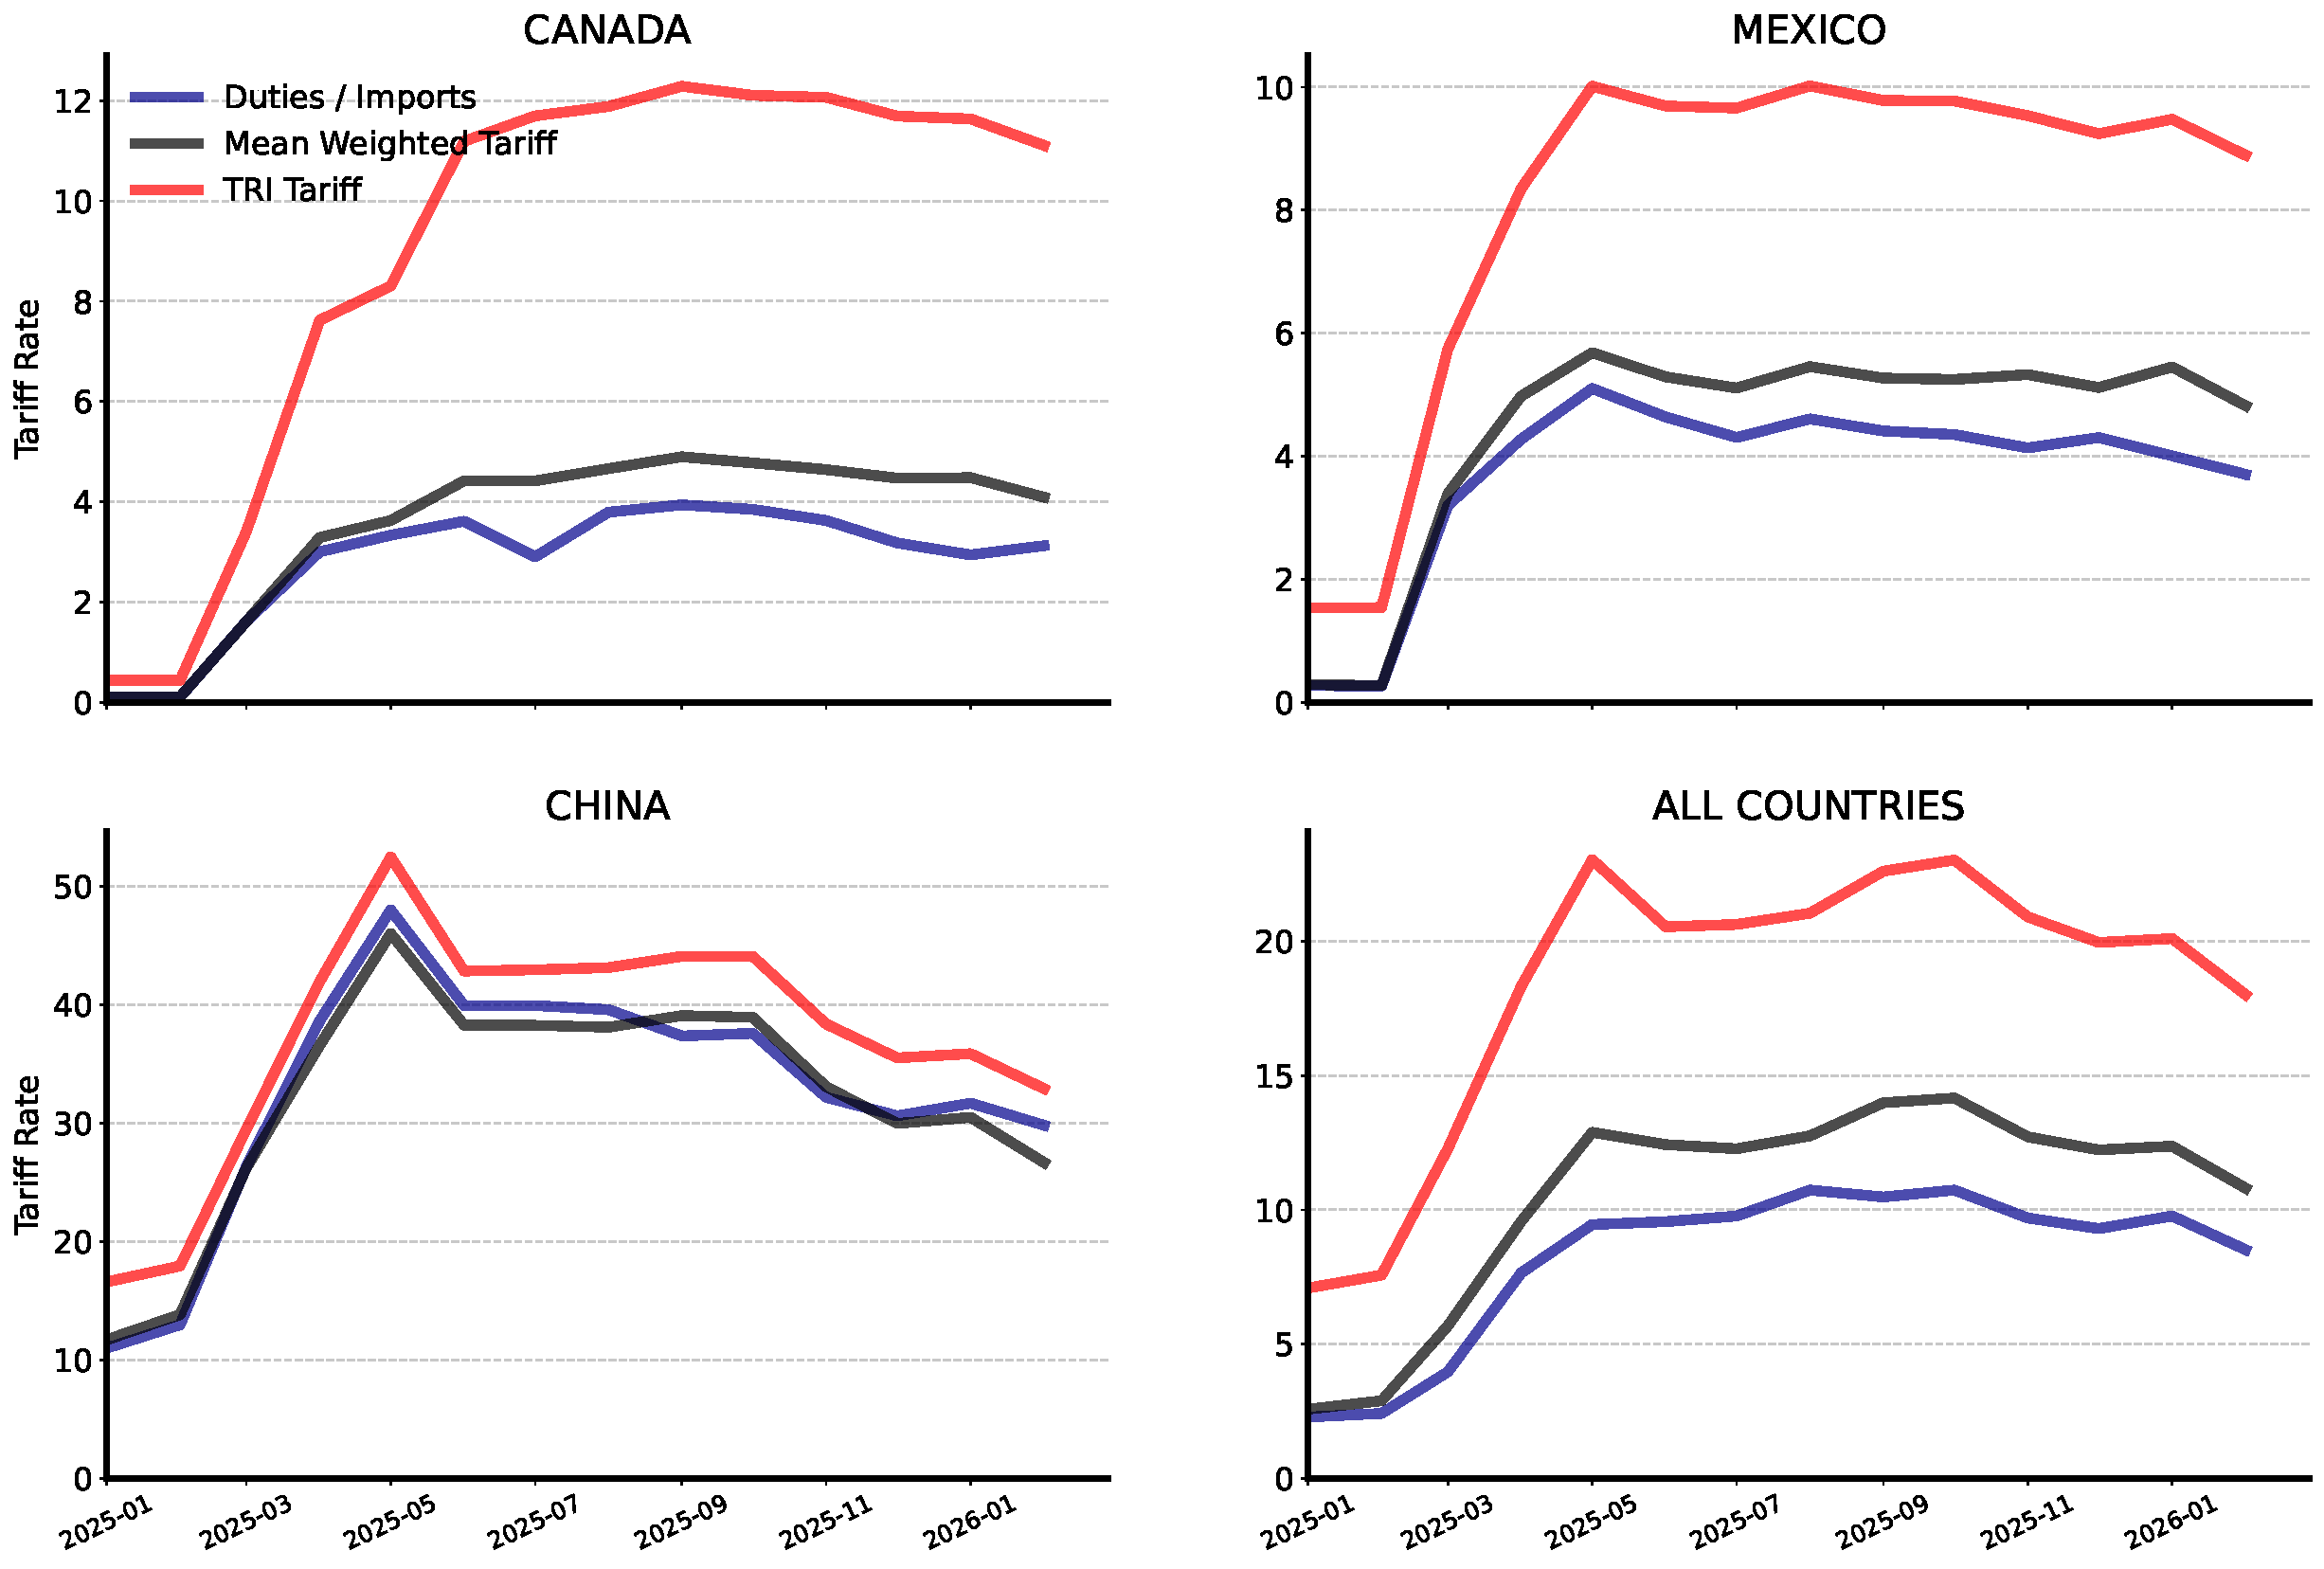
\includegraphics[height=0.95\textheight]{./figures/panel-tariffs.pdf}
\end{figure}
\end{landscape}}

As the top-left panel of Figure \ref{fig:tariff-pannel} shows, Canada is the clearest case where the TRI diverges from average overtariff measures. Since March 2025, the duties/imports tariff rate rises to about \canadasimpleMeanValuetwofive{} percent by \currentdate{}. In contrast, the TRI is \canadarmsValuetwofive{} percent | implying U.S. policy toward Canada is roughly three times more restrictive than what average tariff rates would suggest.

The divergence between the TRI and average tariffs for Canada and Mexico reflects the structure of tariff policy since March 2025. USMCA-compliant goods were exempted from the 25 percent IEEPA tariffs, allowing most trade to continue duty-free. However, automobiles face a 25 percent tariff under Section 232 regardless of USMCA status, and steel and aluminum face tariffs of 50 percent. This divergence reflects a high-dispersion regime: most trade enters at zero (exemptions), while economically important categories face very high tariffs. The TRI captures the welfare cost of that dispersion.

The same issue is apparent for Mexico. Like Canada, average tariff rates have been relatively low. But the large TRI tariff means that U.S. trade policy is much more restrictive towards Mexico | in this case nearly two times more restrictive. Also like Canada, visual inspection of the data shows that autos and auto parts are important categories facing large tariffs, while many imports are coming in near duty free.

China is the opposite, with a relatively small and stable difference between the TRI tariff rate and average tariffs. The distinction here is that there is simply less variance in tariff rates across goods relative to the Canadian or Mexican case.  Yes, the overall level of tariffs is much higher. But tariffs on imports from China don't face the same scale of exemptions that imports from Canada or Mexico do, and thus the TRI tariff measure differs little relative to average tariffs.

Table \ref{tab:tariff_metrics} provides an overview of these tariff metrics as of \currentdate{} for the top 20 U.S. import sources plus the All Country aggregate. In addition to the examples discussed above, Brazil and Switzerland are other countries that stand out with large differences between trade restrictiveness and average tariffs.

\subsection{Trade Restrictiveness By Sector}\label{sec:results3}

The TRIs in (\ref{eq:TRI2}) can also be constructed at sector-level. The sectoral TRI answers the following question: What uniform tariff applied to all goods in a sector would generate the same deadweight loss as the actual tariff structure within that sector?

In constructing the sectoral TRI, a good is defined as a country by HS10 code. The sectoral definition that I focus on is two-digit HS codes. In Figure \ref{fig:sector-tariff-pannel}, I focus on four sectors: Machinery (HS code 84), Electrical Equipment (HS code 85), Vehicles (HS code 87), and Pharmaceuticals (HS code 30). Excluding petroleum and precious metals, these four sectors account for about 50 percent of all U.S. imports.

Figure \ref{fig:sector-tariff-pannel} presents the results. As with the other TRIs, overall restrictiveness is large in three out of four categories. As of \currentdate{}, trade restrictiveness in Machinery, Electrical Equipment, and Vehicles is more or less equivalent to a \rmsValuetwofiveVehicles{} percent tariff.

There is, however, heterogeneity in the magnitude relative to what average tariff measures would suggest. In Machinery, the measure of duties relative to imports would suggest trade is only modestly restricted with a tariff rate of \simpleMeanValuetwofiveMachinery{} percent, substantially below the TRI of \rmsValuetwofiveMachinery{} percent. Electrical Equipment displays a similar pattern.

Vehicles is a counterexample. Here there is less of a gap between the TRI and either the mean weighted tariff of \meanWeightedValuetwofiveVehicles{} or duty measure of \simpleMeanValuetwofiveVehicles{}. This reflects the structure of the Section 232 auto tariffs, which apply broadly across the sector regardless of USMCA status. Unlike Machinery or Electrical Equipment | where cross-country heterogeneity and various exemptions create a mix of low-tariff and high-tariff goods | most vehicle imports face similar tariff rates. Lower dispersion within the sector implies that the TRI and average measures are more similar.

The Vehicle results help explain the country-level patterns documented in Section \ref{sec:results2}. Canada and Mexico are major sources of U.S. vehicle imports, and the high sectoral TRI for Vehicles contributes directly to the elevated TRIs for these countries. At the same time, much of their non-auto trade enters duty-free under USMCA, which keeps average tariffs low. The combination of high sectoral restrictiveness in autos and near-zero tariffs elsewhere drives the large TRI for Canada and Mexico.

\afterpage{%
\clearpage
\begin{landscape}
\begin{figure}
\centering
\caption{Tariff Measures for Selected HS2 Sectors}\label{fig:sector-tariff-pannel}
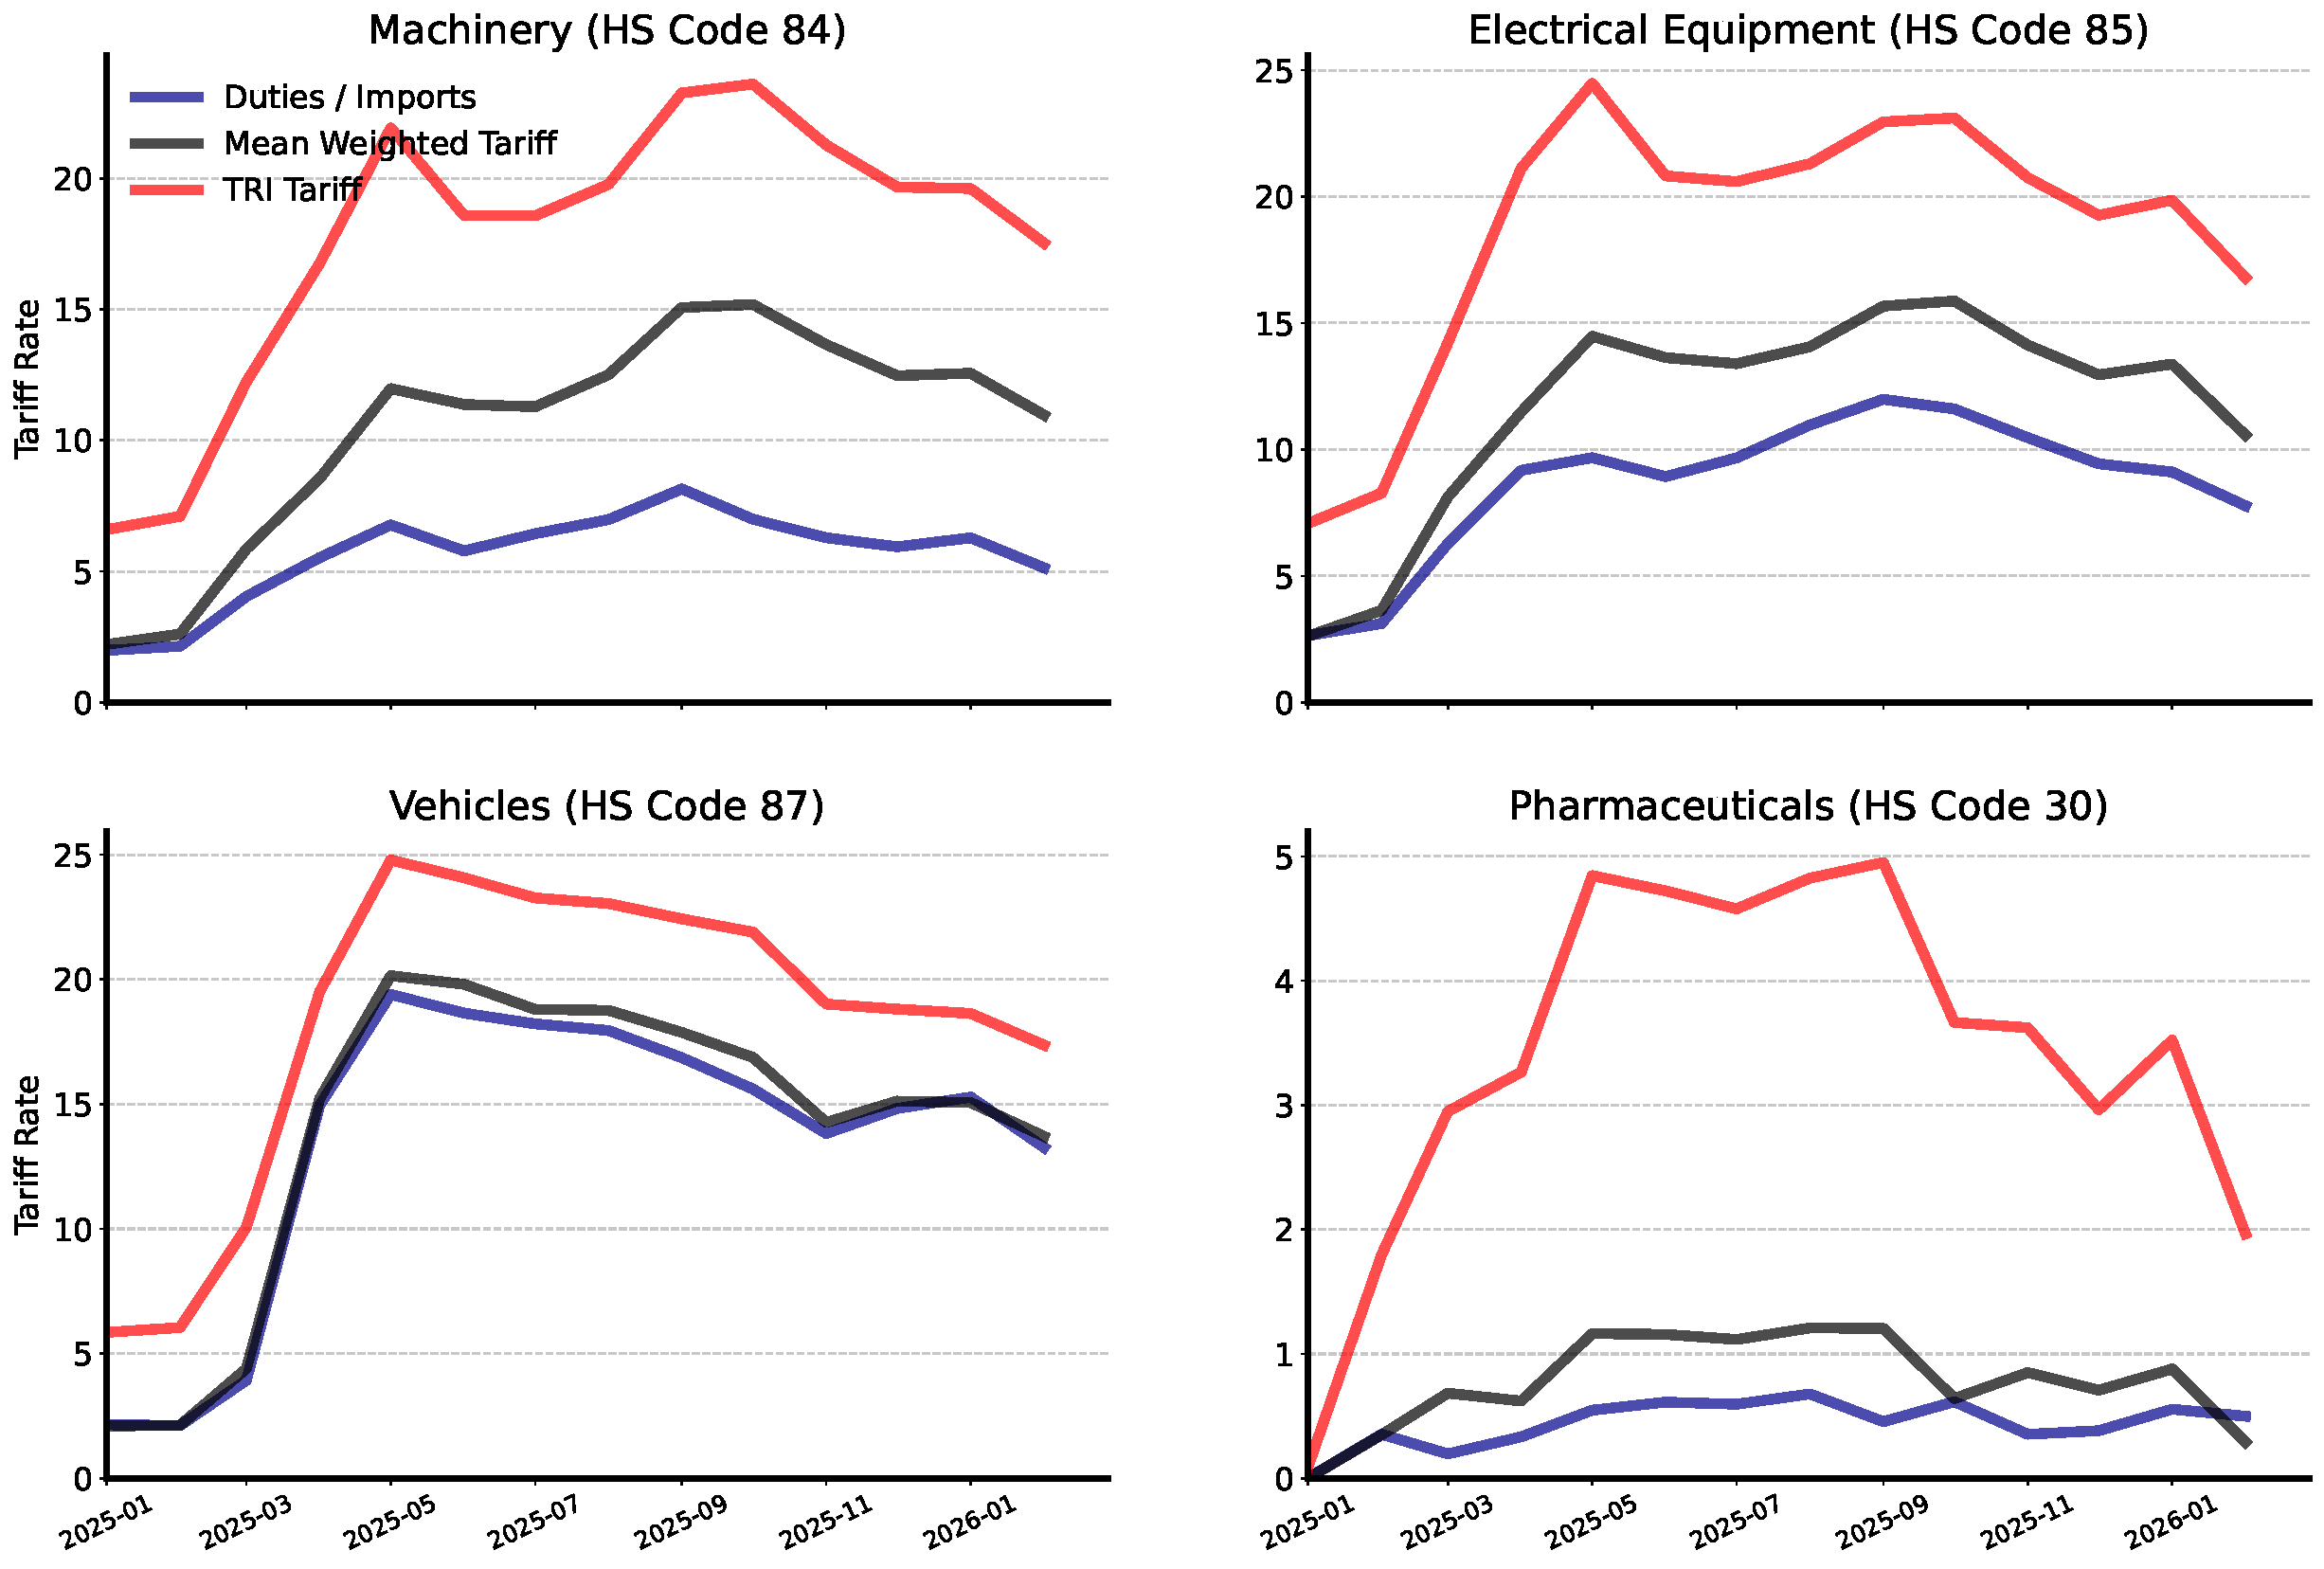
\includegraphics[height=0.95\textheight]{./figures/panel-top-sector-tariffs.pdf}
\end{figure}
\end{landscape}}

The Pharmaceuticals category is where there is a massive difference between the TRI and average measures of tariffs. Overall restrictiveness is modest at \rmsValuetwofivePharmaceuticals{} percent, but this is still larger than the duty measure of near zero suggests. This result lies behind Ireland's low TRI, but large gap between the TRI and average measures (see Table \ref{tab:tariff_metrics}). Approximately half of U.S. imports from Ireland in 2024 are in the Pharmaceutical category.

Another interesting observation is that the scope of substitution differs between sectors. This can be seen in the divergence between the mean weighted tariff and the duty / imports measure. As discussed above, the key distinction between these two measures is that for the mean weighted tariff, the weights are fixed, whereas for the duty measure the weights are changing. Thus, for Vehicles the similarity between the mean weighted and duty measure suggests that changes in sourcing patterns or substitution have been small. However, Machinery and Electrical Equipment display divergence between the mean weighted and duty measure suggesting that substitution is stronger in these categories.

As a summary, Table \ref{tab:tariff_sector} reports the sectoral tariff measures along with informative names and the sector's share of U.S. imports in 2024, excluding petroleum and precious metals.

\section{Conclusion}

Since January 2025, it's become popular for economists, journalists, and policy makers to discuss and track aggregated tariff numbers regarding the current state of U.S. trade policy. However, different tariff regimes are not all created equal | even conditional on having the same average rate of protection.

This short note used the ideas of \citet{anderson1996new, anderson2005measuring} to construct a theoretically grounded measure as to how restrictive U.S. trade policy is. Specifically, I measured the uniform tariff that leaves the U.S. consumer as well off as under actual policy | both in aggregate, by trading partner, and by sector. As the results show, policy has become far more restrictive than what the headline numbers suggest. And these results imply that policy assessments based on average tariffs may be misleading.

With that said, there are important limitations of the analysis. While the measurement is theoretically grounded, I do employ approximations and abstract from details like goods-specific elasticities of trade which may be important. Trade restrictiveness indices only measure how restrictive policy is; they do not quantify the potential inflationary and output costs.

Finally, this is a live document. As newer data are released, the paper here will update and present updated versions of the results.  And the website \url{https://www.tradewartracker.com} will have interactive visualizations of the tariff measures presented here.

\afterpage{%
\clearpage

\begin{table}
\centering
\caption{Tariff Metrics by Sector: December 2025}
\label{tab:tariff_metrics}
\begin{tabular}{lrrr}
\toprule
Country & TRI Tariff & Mean Weighted Tariff & Duties / Imports \\
\midrule
India & 35.9 & 25.7 & 20.4 \\
China & 35.5 & 30.0 & 30.8 \\
Brazil & 27.0 & 15.9 & 14.2 \\
Indonesia & 24.7 & 21.0 & 21.0 \\
Vietnam & 23.0 & 17.9 & 12.5 \\
Thailand & 21.1 & 16.5 & 8.4 \\
All Countries & 20.4 & 12.6 & 9.5 \\
Japan & 17.0 & 13.8 & 13.5 \\
Taiwan & 16.9 & 9.9 & 3.3 \\
Korea, South & 15.8 & 12.0 & 9.3 \\
Malaysia & 15.6 & 10.7 & 10.5 \\
Germany & 15.5 & 11.5 & 9.3 \\
Italy & 14.8 & 10.7 & 11.7 \\
Switzerland & 13.7 & 7.1 & 6.9 \\
Netherlands & 12.5 & 6.8 & 5.1 \\
France & 12.1 & 7.7 & 5.9 \\
Canada & 11.7 & 4.5 & 3.2 \\
Mexico & 9.3 & 5.2 & 4.4 \\
United Kingdom & 9.1 & 6.1 & 7.1 \\
Singapore & 5.6 & 2.3 & 3.0 \\
Ireland & 4.7 & 1.5 & 2.1 \\
\bottomrule
\end{tabular}
\end{table}


}

\afterpage{%
\clearpage
\begin{landscape}
\begin{table}
\centering
\caption{Tariff Metrics by Sector: December 2025}
\label{tab:tariff_sector}
\begin{tabular}{llrrrr}
\toprule
HS2 & HS2 Name & TRI Tariff & Mean Weighted Tariff & Duties / Imports & Share of U.S. Imports \\
\midrule
76 & Aluminum & 44.9 & 39.4 & 40.4 & 0.8 \\
73 & Iron/Steel Articles & 44.5 & 37.7 & 38.4 & 1.5 \\
61 & Knitted Apparel & 43.0 & 40.2 & 39.0 & 1.4 \\
62 & Woven Apparel & 39.6 & 35.7 & 32.4 & 1.1 \\
72 & Iron \& Steel & 38.4 & 31.0 & 29.7 & 1.0 \\
64 & Footwear & 31.7 & 30.0 & 29.2 & 0.8 \\
94 & Furniture & 30.3 & 22.7 & 20.6 & 2.1 \\
40 & Rubber & 24.9 & 18.8 & 16.8 & 1.1 \\
39 & Plastics & 22.3 & 15.2 & 15.2 & 2.2 \\
95 & Toys \& Games & 22.3 & 20.8 & 19.8 & 1.3 \\
84 & Machinery & 19.7 & 12.5 & 6.0 & 15.8 \\
85 & Electrical Equipment & 19.2 & 12.9 & 9.6 & 14.5 \\
87 & Vehicles & 19.0 & 15.4 & 14.9 & 12.0 \\
90 & Optical/Medical Equipment & 16.2 & 11.6 & 10.5 & 3.8 \\
38 & Miscellaneous Chemicals & 14.4 & 8.5 & 12.5 & 0.7 \\
29 & Organic Chemicals & 12.2 & 5.1 & 9.1 & 1.7 \\
22 & Beverages \& Vinegar & 11.9 & 7.5 & 6.6 & 0.9 \\
88 & Aircraft & 10.2 & 4.5 & 3.0 & 1.1 \\
08 & Fruit \& Nuts & 4.9 & 0.7 & 0.5 & 0.7 \\
30 & Pharmaceuticals & 3.0 & 0.7 & 0.4 & 6.7 \\
\bottomrule
\end{tabular}
\end{table}

\end{landscape}
}

\newpage

\bibliography{us-tariff-bibtex}


\newpage

\section*{Appendix: Expenditure-Function Approach to Trade Restrictiveness}

This appendix outlines the duality-based approach behind the Anderson-Neary Trade Restrictiveness Index (TRI) and shows how a second-order Taylor expansion of the expenditure function yields the same root-mean-square (RMS) type expression in (\ref{eq:TRI2}).

\subsection*{A. Expenditure Function and Price Distortions}

For clarity, I'll abstract from the time index in the presentation below. Now define $e(p,u)$ as the expenditure function: the minimum cost of attaining utility $u$ at prices $p$. If the government imposes ad valorem tariffs $\tau = (\tau_1,\ldots,\tau_G)$, consumer prices are
\begin{align}
p^\tau_g = p_g(1+\tau_g).
\end{align}
Equivalent variation of the tariff vector is
\begin{align}
EV(\tau) = e(p^\tau, u^o) - e(p, u^o),
\end{align}
where $u^o$ is the pre-tariff utility level. Now the \emph{uniform tariff} $\hat{\tau}$ is said to be \emph{welfare-equivalent} if
\begin{align}
e(p(1+\hat{\tau}),u^0) = e(p^\tau,u^0),
\end{align}
which is the defining condition of the Trade Restrictiveness Index.

To obtain an analytically tractable expression, expand the expenditure function around the initial prices $p$:
\begin{align}
e(p+\Delta p) \approx e(p) + \sum_g h_g(p)\,\Delta p_g + \frac{1}{2} \sum_{g,{g'}} S_{g{g'}}(p)\,\Delta p_g \Delta p_{g'},
\end{align}
The term $h_g(p) = \partial e/\partial p_g$ is Hicksian (compensated) demand evaluated at initial prices $p$, which follows from Shephard's Lemma. And then the other term: $S_{g{g'}}(p) = \partial^2 e/\partial p_g \partial p_{g'}$ is an element in the Slutsky substitution matrix. And I'm suppressing the notational dependence on the initial level of utility $u^o$.

Now $\Delta p_g = p_g \tau_g$. Thus the welfare change associated with the full tariff vector is approximately
\begin{align}
EV(\tau)
\approx
\sum_g h_g p_g \tau_g
\;+\;
\frac{1}{2} \sum_{g,{g'}} S_{g{g'}} p_g p_{g'} \tau_g \tau_g'.
\end{align}
Evaluating the same expansion for a uniform tariff $\hat{\tau}$ gives
\begin{align}
EV^{uni}(\hat{\tau})
\approx
\hat{\tau} \sum_g h_g p_g
\;+\;
\frac{1}{2} \hat{\tau}^2 \sum_{g,{g'}} S_{g{g'}} p_g p_{g'}.
\end{align}
Then the TRI is the welfare-equivalent uniform tariff which satisfies
\begin{align}
EV(\tau) = EV^{uni}(\hat{\tau}).
\end{align}
To make further progress, I make following simplifications:
\begin{enumerate}
\item Ignore cross-price terms: $S_{gg'}\approx 0$ for $g\neq g'$.

\item Locally approximate Hicksian demand by an isoelastic function. First, the goal is to approximate $S_{gg} p_g^2$ | the curvature of the expenditure function with respect to price $p_g$. By Shephard's lemma, $S_g = h_g$ (compensated demand), so:
\begin{align}
S_{gg} = \frac{\partial h_g}{\partial p_g}
\end{align}
Now assume that compensated demand takes the isoelastic form:
\begin{align}
h_g = A_g p_g^{-\theta_g}
\end{align}
where $\theta_g > 0$ is the (constant) compensated own-price elasticity. Then differentiating with respect to $p_g$:
\begin{align}
\frac{\partial h_g}{\partial p_g} = -\theta_g A_g p_g^{-\theta_g - 1} = -\theta_g \frac{h_g}{p_g}
\end{align}
Finally, multiplying both sides by $p_g^2$ yields
\begin{align}
    S_{gg} p_g^2 \approx -\,\theta_g h_g p_g,
\end{align}
where $\theta_g$ is the compensated elasticity.

\item Match only the second-order terms in the uniform-tariff and vector-tariff expressions. The idea here is that the second-order terms represent the ``true'' efficiency costs of the tariffs. In contrast, the first-order terms (which I'm ignoring) represent transfers from consumers to the government (who then redistribute them back), see, e.g., \citet{feenstra1995estimating}.
    
    The matching only second-order terms deserves more explanation. Notice that the first-order term is:
\begin{align}
    \sum_g h_g(p) \cdot \tau_g p_g
\end{align}
Which is the same as the tariff revenue collected at the initial (pre-tariff) quantities:
\begin{align}
    R \approx \sum_g  h_g(p) \cdot \tau_g p_g 
\end{align}
If this revenue is rebated lump-sum, it is a transfer from the household to the government and back, it does not change total purchasing power. This is the term that ``nets out.'' The second-order term is:
\begin{align}
    \frac{1}{2} \sum_{g,g'} S_{gg'}(p) \tau_g p_g \tau_{g'} p_{g'}
\end{align}
This captures the \textit{substitution} induced by distorted relative prices. Even though the household could afford the original bundle (since revenue is rebated), they choose a different bundle because they face prices $p^\tau$ instead of $p$. This is a pure efficiency loss | no transfer can undo it. 
\end{enumerate}
Under these assumptions:
\begin{align}
\frac{1}{2} \sum_g S_{gg} p_g^2 \hat{\tau_g}^2
=
\frac{1}{2} \sum_g S_{gg} p_g^2 \tau_g^2.
\end{align}
Substituting $S_{gg} p_g^2 \approx -\theta_g h_g p_g$ yields
\begin{align}
\hat{\tau}^2 \sum_g \theta_g h_g p_g
=
\sum_g \theta_g h_g p_g\,\tau_g^2.
\end{align}
And then define
\begin{align}
A = \sum_g \theta_g h_g p_g,
\qquad
\omega_g = \frac{\theta_g h_g p_g}{A}.
\end{align}
Then the welfare-equivalent tariff satisfies
\begin{align}
\hat{\tau} = \sqrt{\sum_g \omega_g \tau_g^2}.
\label{eq:TRI_appendix}
\end{align}
This is identical in form to equation (\ref{eq:TRI1}) in the main text. Then if compensated elasticities are identical across goods, $\theta_g = \bar{\theta}$ and invoking arguments that $h_g p_g$ is approximated by import expenditures, one has
\begin{align}
\omega_g = \frac{\bar{\theta} h_g p_g}{\bar{\theta} \sum_{g'} h_{g'} p_{g'}} = \frac{M_g}{\sum_{g'} M_{g}} = s_g,
\end{align}
where $s_g$ is the share of good $g$ in total import expenditure. In this case, the expenditure-function approach yields the import-share-weighted RMS tariff:
\begin{align}
\hat{\tau}
= \sqrt{\sum_g s_g \tau_g^2},
\end{align}
which matches equation (\ref{eq:TRI2}) in the main text derived using the Harberger welfare-loss formulation.
\end{onehalfspacing}

\end{document}


%\newpage
%
%\begin{landscape}
%\begin{figure}[htbp]
%    \centering
%    \includegraphics[width=\linewidth]{./figures/unilateral-tariff.pdf}
%    \caption{U.S. Unilateral Tariff}
%    \label{fig:unilateral}
%\end{figure}
%\end{landscape}

%\newpage




%\smallskip
%\item
%\smallskip
%\item $\log$ for $u$ and iso-elastic disutility of labor with a Frisch elasticity of 0.50.
%\smallskip
%\item Discount rate picked to target an annual interest rate of one percent.
%\smallskip
%\item Capital shares and depreciation are standard values.
%\smallskip
%\item
%\smallskip
%\item Trade elasticity set to 4.0.
%\smallskip
%\item Trade costs set to target a home trade share of 80 percent.




%%\begin{align}
%%\frac{p_{ij'}^{1-\theta}}{\sum\limits_{j} p_{ij}^{1-\theta}} = \pi_{ij}.
%%\end{align}
%
%
%Capital demand is determined from the firms first order condition with
%\begin{align}
%\bigg( \frac{ p_{iit} }{P_{I,it}} \bigg) \alpha A_{i} K_{it}^{\alpha - 1}N_{it}^{1-\alpha} = r_{kt}.
%\label{eq:marginal-product-capital}
%\end{align}
%This is relatively standard, however, it is worth thinking through the units here which I describe in depth below.
%
%The non-bracketed part on the left-hand side describes the physical marginal product of capital, i.e., how many extra units of good $i$ given an extra unit of physical capital. When this is multiplied by $p_{iit}$ or the price of good $i$, it now describes how many units of the numeraire are delivered given an extra unit of capital.\footnote{Notice that given the ice-berg structure of trade costs, it's sufficient to simply work with the prevailing domestic price of good $i$.} This price then divides through by $P_{I,it}$ or the price of investment in country $i$ which describes how many units of capital a unit of numeraire can acquire in country $i$.  Thus, the entire left hand side describes how many extra units of the numeraire are returned given one unit of the numeraire invested in capital. And this equals the rental rate of capital in the correct units, $r_{kt}$.
%
%What's interesting here is how one can see the influence of the terms of trade and what a tariff may do. One the one hand, a tariff will have a beneficial effect by improving the terms of trade. By making the value of a countries commodity, i.e., $p_{iit}$ scarce, the tariff increases the value of the marginal product of capital and would induce an inflow of capital to the country and raise output. One the other hand, the tariff has the effect of \emph{lowering} capital demand by making investment more expensive with an increase in $P_{I,it}$.


%\section{Characterization, National Accounting, and Equilibrium}
%
%This section characterizes key conditions that the firm and household optimization problems must satisfy. We then discuss how the model is consistent with both the standard National Incompe and Product (NIPA) accounting identifies and the Balance of Payments accounting. We then define and equilibrium.
%
%\subsection{Goods Prices}
%
%Given the trade frictions and competition in production, the price for country $i$ to purchase a good from location $j$ is
%\begin{align}
%p_{ijt} = (1 + \tau_{ijt}) d_{ijt} \Bigg( \frac{ r_{kt}^{\alpha}w_{jt}^{1-\alpha}}{A_{jt}} \Bigg ).
%\label{eq:marginal-product-ship}
%\end{align}
%This is the standard relationship connecting the unit marginal cost of production in country $j$, trade costs, and then tariffs which determines the prices that consumers and firms face when importing goods.
%
%\subsection{Capital and Labor Demand}
%
%Capital and labor demand come from the firms's side of the economy.
%
%Capital demand is determined from the firms first order condition with
%\begin{align}
%\bigg( \frac{ p_{iit} }{P_{I,it}} \bigg) \alpha A_{i} K_{it}^{\alpha - 1}N_{it}^{1-\alpha} = r_{kt}.
%\label{eq:marginal-product-capital}
%\end{align}
%This is relatively standard, however, it is worth thinking through the units here which I describe in depth below.
%
%The non-bracketed part on the left-hand side describes the physical marginal product of capital, i.e., how many extra units of good $i$ given an extra unit of physical capital. When this is multiplied by $p_{iit}$ or the price of good $i$, it now describes how many units of the numeraire are delivered given an extra unit of capital.\footnote{Notice that given the ice-berg structure of trade costs, it's sufficient to simply work with the prevailing domestic price of good $i$.} This price then divides through by $P_{I,it}$ or the price of investment in country $i$ which describes how many units of capital a unit of numeraire can acquire in country $i$.  Thus, the entire left hand side describes how many extra units of the numeraire are returned given one unit of the numeraire invested in capital. And this equals the rental rate of capital in the correct units, $r_{kt}$.
%
%What's interesting here is how one can see the influence of the terms of trade and what a tariff may do. One the one hand, a tariff will have a beneficial effect by improving the terms of trade. By making the value of a countries commodity, i.e., $p_{iit}$ scarce, the tariff increases the value of the marginal product of capital and would induce an inflow of capital to the country and raise output. One the other hand, the tariff has the effect of \emph{lowering} capital demand by making investment more expensive with an increase in $P_{I,it}$.
%
%Labor demand follows from a similar first order condition with
%\begin{align}
%p_{iit} (1-\alpha) A_{i} K_{it}^{\alpha}N_{it}^{-\alpha} = w_{it}.
%\end{align}
%Again, thinking through the units is helpful: the part on the left hand side without the price is the physical marginal product of labor, i.e. how many extra units of good $i$ given an extra unit of labor. And then this is multiplied by the price of good $i$ which tells us how many units of the numeraire are delivered given an extra unit of labor. And this must equal the wage rate which is how many extra units of the numeraire the household receives given an extra unit of labor is supplied. So the value of the marginal product of labor should be equal to the wage.
%
%\subsection{Capital and Labor Supply}
%
%Capital and labor supply come from the households problem.
%
%The household side of the problem is characterized by several equations. First, the household sets consumption equal to the marginal utility of wealth with
%\begin{align}
%\frac{ u'(c_{it}(a,z)), n_{it}(a,z)}{P_{it}}= \lambda_{it}(a,z)
%\end{align}
%where $P_{it}$ is the ideal price index of consumption in country $i$. Given the CES aggregator across varieties, this price index is
%\begin{align}
%P_{it} = \bigg[ \sum\limits_{j\in M} p_{ijt}^{1-\theta} \bigg]^{\frac{1}{1 - \theta}}.
%\end{align}
%Consumption expenditure across different varieties is given by
%\begin{align}
%\frac{p_{ij'}^{1-\theta}}{\sum\limits_{j} p_{ij}^{1-\theta}} = \pi_{ij}.
%\end{align}
%
%
%The Euler equation (for households away from the borrowing constraint) relates consumption today with consumption tomorrow where
%\begin{align}
%\lambda_{i}(a,z) = \beta R \mathbb{E}  \lambda_{i}(a',z')
%\end{align}
%which equates the marginal utility of wealth across time periods. This implicitly defines an savings policy function for households, and thus when aggregating all households determines their asset supply to the global intermediaries. Finally, with the GHH labor supply, the labor supply is
%\begin{align}
%n_{i} = \bigg( \frac{w_{i}}{P_{i}} \bigg)^{\varphi}.
%\end{align}
%which is simply a function of the real wage in country $i$.
%
%
%
%\subsection{Trade}
%
%The CES-Armington structure makes things relatively simple. Moreover, because of the consumption aggregator and investment aggregator are the same it is even simpler.
%
%The share of expenditure in $i$ on goods from $j$ is given by
%\begin{align}
%\frac{p_{ij'}^{1-\theta}}{\sum\limits_{j} p_{ij}^{1-\theta}} = \pi_{ij}.
%\end{align}
%where notice that the sum of $\pi_{ij}$ across $j$ must equal one. This then implies that imports are given by
%\begin{align}
%\mbox{Imports}_{ij} = \pi_{ij} P_{it} \bigg[ \int c^k_{it} dk \  +  I_{it} \bigg]
%\end{align}
%where the first term in the brackets is total consumption expenditure by all households and the second term is investment demand by firms.
%
%
%\section{National Income and Balance of Payment Accounting}
%
%I'm just going to walk through some accoutring concepts, especially with respect to balance of payment issues, so they are clear.
%
%\subsection{National Income Accounting Identity}
%First, lets derive the national accounting identities. First, we have the following where
%\begin{align}
%p_{iit} A_{i} K_{it}^{\alpha} N_{it}^{1-\alpha} =  p_{iit} \int c^k_{iit} dk \ + p_{ii} I_{iit} \ + \ \sum_{j\neq i} \frac{p_{jit}}{1+ \tau_{jit}} \int c^k_{jit} dk + \sum_{j\neq i} \frac{p_{jit}}{1+ \tau_{jit}} I_{jit}
%\label{eq:goods-market-clearing}
%\end{align}
%or the value of production must equal the value of domestic consumption plus the value of domestic investment goods, plus exports, not including the foreign tariffs. Before moving on, this is one of the equilibrium conditions that must be satisfied: the value of production must equal the value of consumption globally which is equal to domestic spending on the good plus exports.
%
%
%Now to get towards the National Income identity, we have a relationship for private consumption which is
%\begin{align}
%P_{it}C_{it} = p_{iit} \int c^k_{iit} dk + \ \sum_{j\neq i} \frac{p_{ijt}}{1+ \tau_{ijt}} \int c^k_{ijt} dk
%\end{align}
%and then we have a relationship for investment which is
%\begin{align}
%P_{it}I_{it} = p_{iit} I_{iit} + \ \sum_{j\neq i} \frac{p_{ijt}}{1+ \tau_{ijt}} I_{ijt}
%\end{align}
%and then combining this we have the traditional $Y = C+ \dots$ equation we get
%\begin{align}
%\underbrace{p_{iit} A_{i} K_{it}^{\alpha} N_{it}^{1-\alpha} \phantom{\int}}_{\mbox{GDP}} & = \label{eq:gdp-identity} \\
%\nonumber \\
%& P_{it}C_{it} \ + \  P_{it}I_{it} + \ \underbrace{\sum_{j\neq i} \frac{p_{jit}}{1+ \tau_{jit}} \int c^k_{jit} dk + \sum_{j\neq i} \frac{p_{jit}}{1+ \tau_{jit}} I_{jit}}_{\mbox{Exports}} -  \ \underbrace{\sum_{j\neq i} \frac{p_{ijt}}{1+ \tau_{ijt}} \int c^k_{ijt} dk - \sum_{j\neq i} \frac{p_{ijt}}{1+ \tau_{ijt}} I_{ijt}}_{\mbox{Imports}} \nonumber
%\end{align}
%
%\subsection{Balance of Payment Accounting}
%So work from the households budget constraint and aggregate across all households where
%\begin{align}
%\sum_{j} p_{ijt} \int c^k_{ijt} dk = w_{it}N_{it} + \mathcal{A}_{it}R_{t} - \mathcal{A}_{it+1} + L_{i} T_{it} \\
%\nonumber \\
%p_{iit} \int c^k_{iit} dk + \ \sum_{j\neq i} \frac{p_{ijt}}{1+ \tau_{ijt}} \int c^k_{ijt} dk +  \sum_{j\neq i} \frac{\tau_{ijt} p_{ijt}}{1+ \tau_{ijt}} \int c^k_{ijt} dk = w_{it}N_{it} + \mathcal{A}_{it}R_{t} - \mathcal{A}_{it+1} + L_{i} T_{it}
%\end{align}
%where $\mathcal{A}_{it}$ is aggregate asset holdings in the economy, and the last line broke out what is going towards taxes and what is not. Then using the governments budget constraint we have
%\begin{align}
%p_{iit} \int c^k_{iit} dk + \ \sum_{j\neq i} \frac{p_{ijt}}{1+ \tau_{ijt}} \int c^k_{ijt} dk  = w_{it}N_{it} + \mathcal{A}_{it}R_{t} - \mathcal{A}_{i+1} - \sum_{j\neq i} \frac{\tau_{ijt} p_{ijt}}{1+ \tau_{ijt}} I_{ijt}
%\end{align}
%Now we are going to add and subtract on both sides of this equation investment and capital income to be able to line this up with GDP. So we have
%\begin{align}
%P_{it}C_{it} + P_{it}I_{i}  = w_{it}N_{it} + r_{kt}P_{it}K_{it} + \mathcal{A}_{it}R_{t} - \mathcal{A}_{it+1} + P_{it}[K_{it+1} + (1- \delta)K_{it}] - r_{kt}P_{it}K_{it}
%\end{align}
%And notice how this is just simply adding and subtracting stuff (and because I have investment expenditure on the left hand side, I'm able to kill the tariff revenue part coming from investment goods). Let's check units again. So the left hand side is in the units of the numeraire. The right hand side too\ldots this is why I have $P_{it}K_{it}$ in these spots which reflects the value of the capital stock in country $i$, in the units of the numeraire. So everything is all good.
%
%We know that payments to capital must equal the value of production so
%\begin{align}
%P_{it}C_{it} + P_{it}I_{i}  = p_{iit} A_{i} K_{it}^{\alpha} N_{it}^{1-\alpha} + \mathcal{A}_{it}R_{t} - \mathcal{A}_{it+1} + P_{it}[K_{it+1} + (1- \delta)K_{it}] - r_{kt}P_{it}K_{it}
%\end{align}
%and then we have the following
%\begin{align}
%GDP_{it} - P_{it}C_{it} -  P_{it}I_{i} = -\mathcal{A}_{it}R_{t} + \mathcal{A}_{it+1} - P_{it}[K_{it+1} + (1- \delta)K_{it}] + r_{kt}K_{it}
%\end{align}
%then lining this up with the GDP identity in (\ref{eq:gdp-identity}) we have
%\begin{align}
%\mbox{Exports}_{it} \ - \   \ \mbox{Imports}_{it} \ =  \ -\mathcal{A}_{it}R_{t} + \mathcal{A}_{it+1} - P_{it}[K_{it+1} + (1- \delta)K_{it}] + r_{kt}P_{it}K_{it}
%\end{align}
%where we need to remember that both exports and imports are exclusive of the tariffs. Then lets rearrange this to get towards traditional balance of payment language where
%\begin{align}
%\underbrace{ \underbrace{ \Bigg [ \mbox{Exports}_{it} \ - \   \ \mbox{Imports}_{it}\Bigg ]}_{\mbox{Trade Deficit}}  \ + \underbrace{ \Bigg[ r_{t}(\mathcal{A}_{it} - P_{it}K_{it})\Bigg] }_{\mbox{NFI}} }_{\mbox{Current Account}} \ = \ \underbrace{\Bigg[ (\mathcal{A}_{it+1} - \mathcal{A}_{it}) - P_{it}(K_{it+1} - K_{it}) \bigg]}_{\Delta\mbox{NFA}}
%\end{align}
%where the last step was to connect $r_{kt}$ with $r_{t}$ and then pull the depreciation term into the change in the net foreign asset position. This is the is the main BoP equation. And finally notice that the NFA position is
%\begin{align}
%\mbox{NFA}_{it} = \mathcal{A}_{it} - P_{it} K_{it}
%\end{align}
%which is the difference between the savings from the household at the value of capital stock in country $i$.
%
%What does this mean? First, notice there can be trade deficits in a stationary setting. There can not be current account deficits. Off from a stationary setting, lets walk through several cases:
%\begin{itemize}
%\item The non-stationary case is the easier to think about. So suppose that initially, $\mathcal{A}_{it} - K_{it} = 0$ and that we start running a trade deficit. This meas that investing demand must be increasing more than how our savings are changing.
%
%\item Similarly, suppose we start running a trade surplus, this implies that we are accumulating assets relative to domestic investments because we are producing more than we are consuming.
%\end{itemize}
%Also notice how this collapses in the closed economy. In the closed economy, now the price of consumption (and investment) can be set to one, it's the numeraire. Them $\mathcal{A}_{it} = K_{it}$ and we have our classic Ayagari economy.
%
%
%\subsection{Equilibrium}
%
%I've already outlined that we have a goods market clearing condition which is given in (\ref{eq:goods-market-clearing}). The prices effectively determining these conditions are the wages in each county. Then we have a global asset market clearing condition which requires that
%\begin{align}
%\sum_{j\in M} \mathcal{A}_{jt} =  \sum_{j\in M}  P_{jt} K_{jt}
%\end{align}
%or that the sum of global net foreign assets is zero. Then associated with this condition, there is a world return on assets $r$ which is moved around to clear this market.





